\documentclass[pointlessnumbers, abstracton, headsepline, a4paper]{scrartcl}

\usepackage[T1]{fontenc}
\usepackage[utf8]{inputenc}
\usepackage{graphicx}
\usepackage{microtype}
\usepackage{textcomp}
\usepackage{ellipsis, fixltx2e, mparhack, booktabs, longtable}
\usepackage[automark]{scrpage2}
\usepackage{multicol}
\usepackage{microtype}
\usepackage{listings}
\usepackage[a4paper]{geometry}
\usepackage[polish]{babel}
\usepackage{subfigure}

\usepackage{courier}
\lstset{
         basicstyle=\footnotesize\ttfamily, % Standardschrift
         %numbers=left,               % Ort der Zeilennummern
         numberstyle=\tiny,          % Stil der Zeilennummern
         %stepnumber=2,               % Abstand zwischen den Zeilennummern
         numbersep=5pt,              % Abstand der Nummern zum Text
         tabsize=2,                  % Groesse von Tabs
         extendedchars=true,         %
         breaklines=true,            % Zeilen werden Umgebrochen
         keywordstyle=\color{red},
         stringstyle=\color{white}\ttfamily, % Farbe der String
         showspaces=false,           % Leerzeichen anzeigen ?
         showtabs=false,             % Tabs anzeigen ?
         showstringspaces=false      % Leerzeichen in Strings anzeigen ?        
}

% part of the hyperref bundle
\usepackage{ifpdf}

\geometry{verbose,tmargin=3.5cm,bmargin=3.5cm}
\setlength{\parskip}{\medskipamount}
\setlength{\parindent}{0pt}

\clearscrheadfoot
\ohead{\\\headmark}
\ihead{
\includegraphics[scale=0.2]{img/zut2.jpg}}
\ofoot[\pagemark]{\pagemark}

% if pdflatex is used
\ifpdf

%set fonts for nicer pdf view
\IfFileExists{lmodern.sty}{\usepackage{lmodern}}
  {\usepackage[scaled=0.92]{helvet}
    \usepackage{mathptmx}
    \usepackage{courier} }
\fi

% the pages of the TOC are numbered roman
% and a pdf-bookmark for the TOC is added
\pagenumbering{arabic}
\let\myTOC\tableofcontents
\renewcommand\tableofcontents{\myTOC\clearpage\pagenumbering{arabic}}

\begin{document}
\begin{titlepage}

\begin{center}

\includegraphics[scale=0.5]{logos/zut.jpg}
\par
\end{center}

\begin{center}
\textsf{\textbf{\LARGE Wydział Informatyki}}
\end{center}{\LARGE}

\vspace{1.5cm}

\begin{center}
\textsf{\Large Metody sztucznej inteligencji}
\end{center}

\begin{center}
\textsf{\textbf{\Large Laboratorium 01 IUz-22 Urbaniak}}
\end{center}

\begin{center}
\textsf{\large Sprawozdanie}
\end{center}

\vspace{3.5cm}

\begin{center}
\begin{tabular}{ll}
Autor: & Sergiusz Urbaniak\tabularnewline
Grupa: & IUz-22\tabularnewline
Data: & \today\tabularnewline
\end{tabular}
\end{center}

\end{titlepage}

\tableofcontents

\section{Bramki logiczne}
\subsection{Bramka OR}

Bramka OR posiada tablice prawdy pokazaną w tablicy \ref{tab:or}.

\begin{table}[h]
\centering
\begin{tabular}[t]{c|c}
Wejście & Wyjście \\
\hline
0 0 & 0 \\
0 1 & 1 \\
1 0 & 1 \\
1 1 & 1 \\
\end{tabular}
\caption{\label{tab:or}Tablica prawdy bramki OR}
\end{table}

Wartości wejściowe są wpisane do zmiennej \texttt{we}. Dane wyjściowe według tablicy prawdy \ref{tab:or} są wpisane w zmienną \texttt{wy}. Następnie jest tworzona ``sieć'' jednego perceptronu i przeprowadzona symulacja działania sieci bez uczenia perceptronu. Kod źródłowy jest dostępny w listingu \ref{lst:or_unteached}.

\begin{center}
\begin{minipage}{0.5\textwidth}
\lstset{captionpos=b,caption=Kod nie uczonej bramki OR,label=lst:or_unteached}
\lstinputlisting{src/or_unteached.m}
\end{minipage}
\end{center}

Wykres błędu jak i danych generowany kodu \ref{lst:or_unteached} jest widoczny na rysunkach \ref{fig:or}.

\begin{figure}[!h]
\centering
\subfigure[Wykres błędu (nie uczone)]{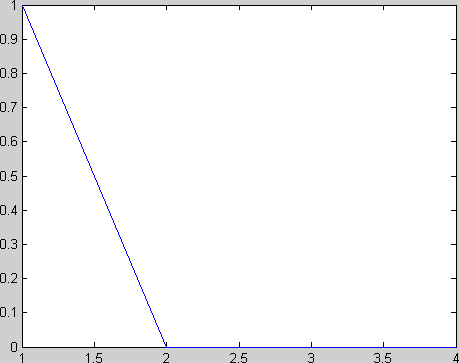
\includegraphics[scale=0.4]{figures/or_error_unlearned.png}}
\subfigure[Linia podziału (nie uczone)]{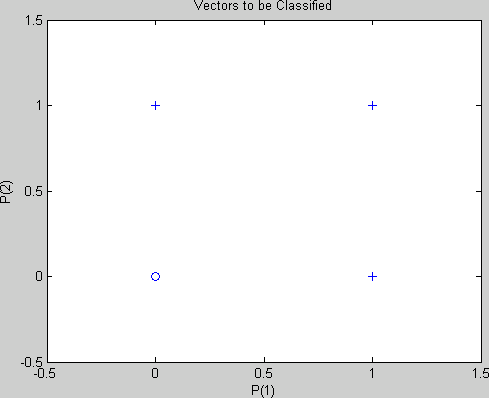
\includegraphics[scale=0.4]{figures/or_data_unlearned.png}}
\subfigure[Wykres błędu (uczone)]{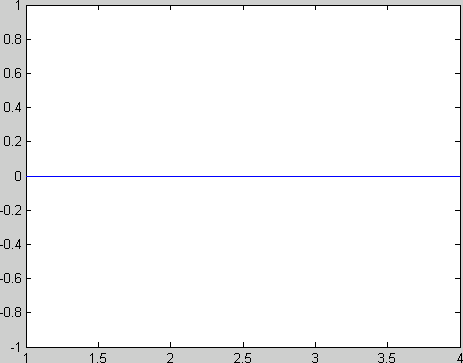
\includegraphics[scale=0.4]{figures/or_error_learned.png}}
\subfigure[Linia podziału (uczone)]{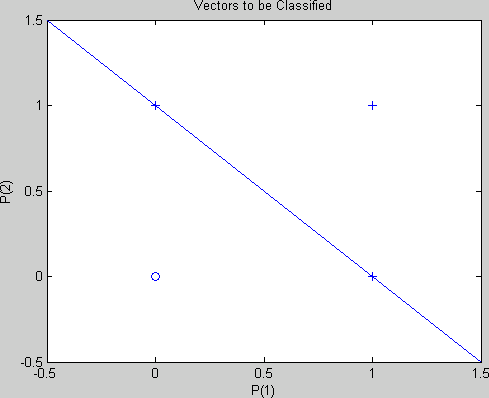
\includegraphics[scale=0.4]{figures/or_data_learned.png}}
\caption{\label{fig:or}Wykresy bramki OR}
\end{figure}

Kod zmieniony na uczenie perceptronu jest widoczny w listingu \ref{lst:or_teached}. Dodane zostały polecenia \texttt{init} i \texttt{train}.

\begin{center}
\begin{minipage}{0.5\textwidth}
\lstset{captionpos=b,caption=Kod uczonej bramki OR,label=lst:or_teached}
\lstinputlisting{src/or_teached.m}
\end{minipage}
\end{center}

Można zaobserwować że uczenie nie pozostawiło żadnego błędu. Perceptron poprawnie nauczył się bramki OR.

\subsection{Bramka XOR}

Bramka XOR posiada tablice prawdy pokazaną w tablicy \ref{tab:xor}.

\begin{table}[h]
\centering
\begin{tabular}[t]{c|c}
Wejście & Wyjście \\
\hline
0 0 & 0 \\
0 1 & 1 \\
1 0 & 1 \\
1 1 & 0 \\
\end{tabular}
\caption{\label{tab:xor}Tablica prawdy bramki XOR}
\end{table}

Kod perceptronu nie uczonego jest widoczny w listingu \ref{lst:xor_unteached}. Jak widać została tylko zmieniona zmienna \texttt{wy}.

\begin{center}
\begin{minipage}{0.5\textwidth}
\lstset{captionpos=b,caption=Kod nie uczonej bramki XOR,label=lst:xor_unteached}
\lstinputlisting{src/xor_unteached.m}
\end{minipage}
\end{center}

Wykres błędu jak i danych generowany kodu \ref{lst:xor_unteached} jest widoczny na rysunkach \ref{fig:xor}.

\begin{figure}[!h]
\centering
\subfigure[Wykres błędu (nie uczone)]{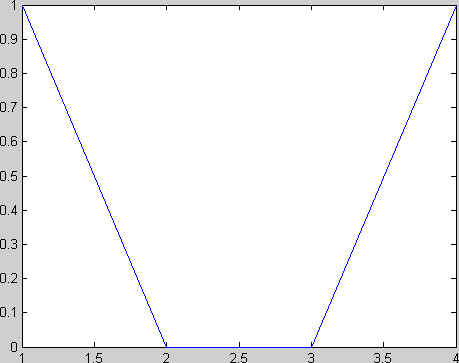
\includegraphics[scale=0.4]{figures/xor_error_unlearned.png}}
\subfigure[Linia podziału (nie uczone)]{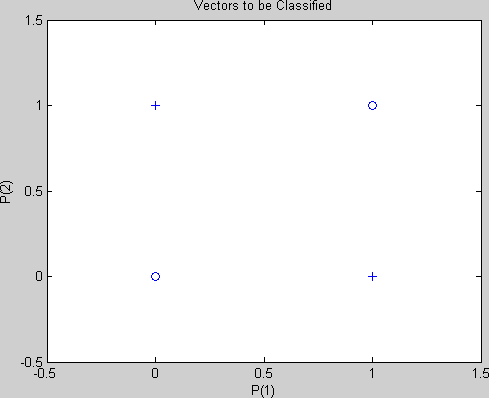
\includegraphics[scale=0.4]{figures/xor_data_unlearned.png}}
\subfigure[Wykres błędu (uczone)]{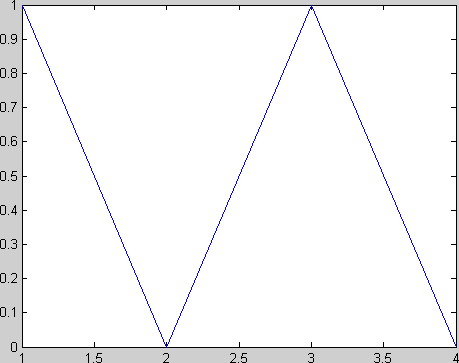
\includegraphics[scale=0.4]{figures/xor_error_learned.png}}
\subfigure[Linia podziału (uczone)]{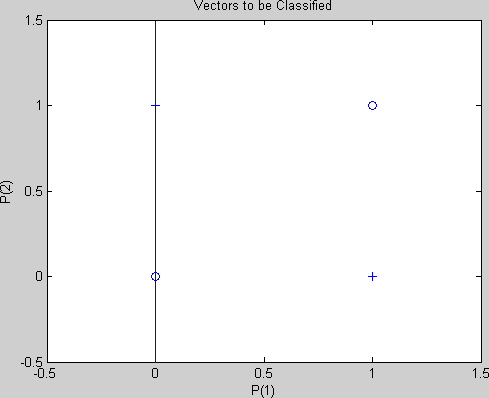
\includegraphics[scale=0.4]{figures/xor_data_learned.png}}
\caption{\label{fig:xor}Wykresy bramki XOR}
\end{figure}

Kod zmieniony na uczenie perceptronu jest widoczny w listingu \ref{lst:xor_teached}. Znów dodane zostały polecenia \texttt{init} i \texttt{train}.

\begin{center}
\begin{minipage}{0.5\textwidth}
\lstset{captionpos=b,caption=Kod uczonej bramki XOR,label=lst:xor_teached}
\lstinputlisting{src/xor_teached.m}
\end{minipage}
\end{center}

Można zaobserwować że uczenie nie udało się. Nadal istnieją błędy. Powodem jest fakt że podział danych bramki XOR nie jest lineowo separowalny.

\clearpage
\section{Dane wczytane z plików}

Aby ułatwić generowanie i wczytanie dużej ilości wykresów został stworzony nowy skrypt widoczny w listingu \ref{lst:load_learn_plot}. Ten skrypt bierze jako parametr prefiks sprawdzanych danych \texttt{prefix}. Na podstawie prefiksu są wczytane dane z plików \texttt{[prefix '\_i.txt']} i \texttt{[prefix '\_o.txt']}. Zmienna \texttt{learn} podaje czy neuron ma być uczony czy nie. W końcu zmienna \texttt{epochs} specyfikuje ile epok uczenia mają być uwzględnione.

\begin{center}
\begin{minipage}{0.8\textwidth}
\lstset{captionpos=b,caption={\texttt{load\_learn\_plot.m}: Kod do wczytania, uczenia i generowania wykresów},label=lst:load_learn_plot}
\lstinputlisting{src/load_learn_plot.m}
\end{minipage}
\end{center}

Wykresy generowane są widoczne w następujących stronach.

\begin{figure}[!h]
\centering
\subfigure[Wykres błędu (nie uczone)]{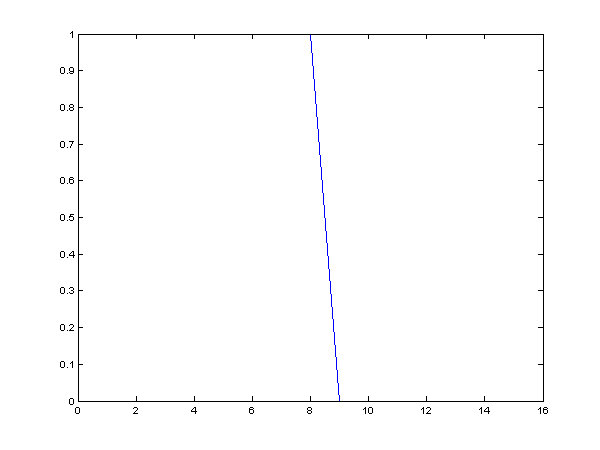
\includegraphics[scale=0.7]{figures/percep_error_unlearned.png}}
\subfigure[Wykres błędu (uczone)]{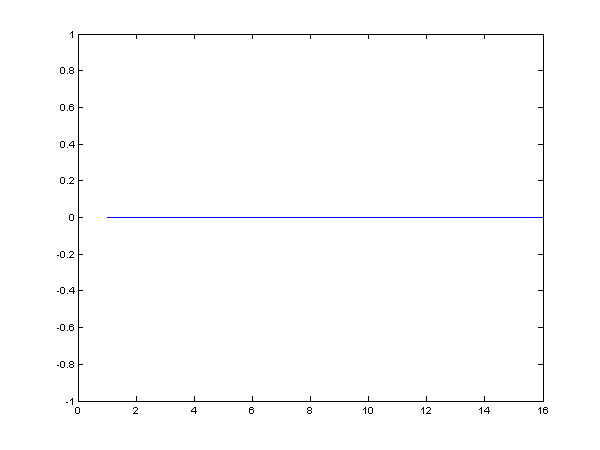
\includegraphics[scale=0.7]{figures/percep_error_learned.png}}
\caption{\label{fig:percep_error}Wykresy błędu zestawu danych \texttt{percep}}
\end{figure}

\begin{figure}[!h]
\centering
\subfigure[Linia podziału (nie uczone)]{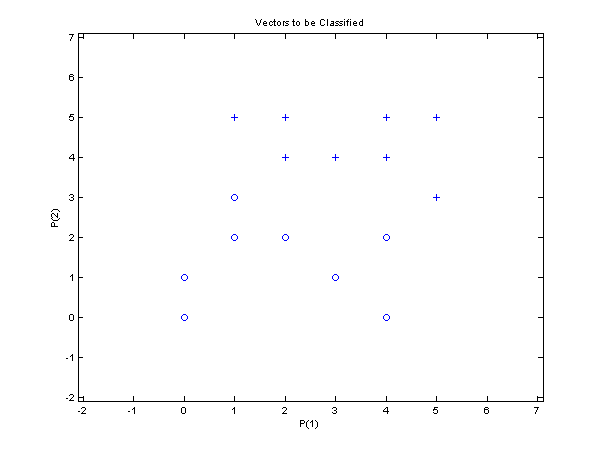
\includegraphics[scale=0.7]{figures/percep_data_unlearned.png}}
\subfigure[Linia podziału (uczone)]{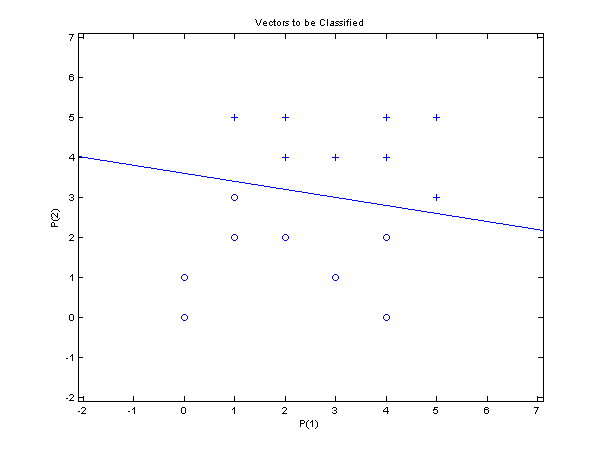
\includegraphics[scale=0.7]{figures/percep_data_learned.png}}
\caption{\label{fig:percep_data}Wykresy przedziału zestawu danych \texttt{percep}}
\end{figure}

\begin{figure}[!h]
\centering
\subfigure[Wykres błędu (nie uczone)]{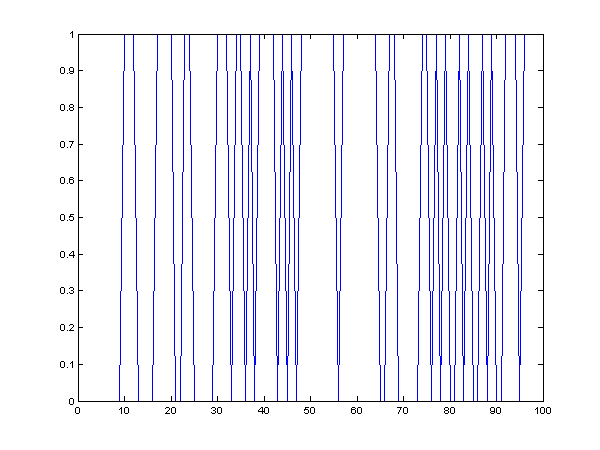
\includegraphics[scale=0.7]{figures/dane_a_error_unlearned.png}}
\subfigure[Wykres błędu (uczone)]{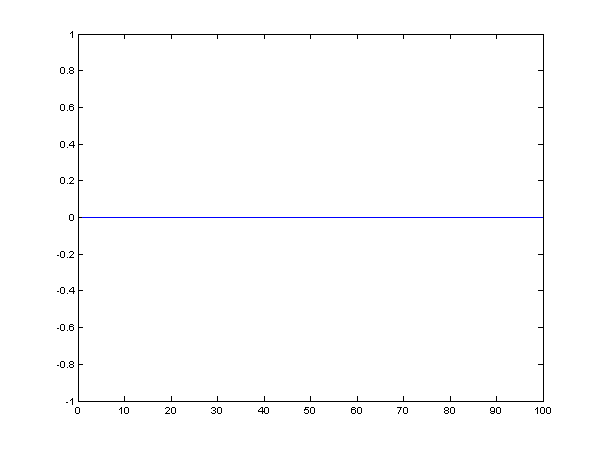
\includegraphics[scale=0.7]{figures/dane_a_error_learned.png}}
\caption{\label{fig:dane_a_error}Wykresy błędu zestawu danych \texttt{dane\_a}}
\end{figure}

\begin{figure}[!h]
\centering
\subfigure[Linia podziału (nie uczone)]{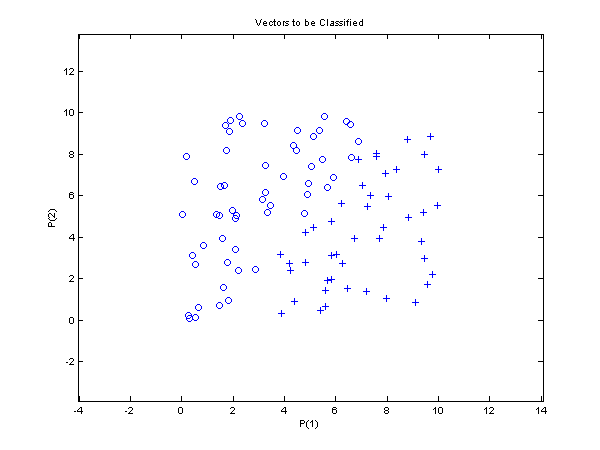
\includegraphics[scale=0.7]{figures/dane_a_data_unlearned.png}}
\subfigure[Linia podziału (uczone)]{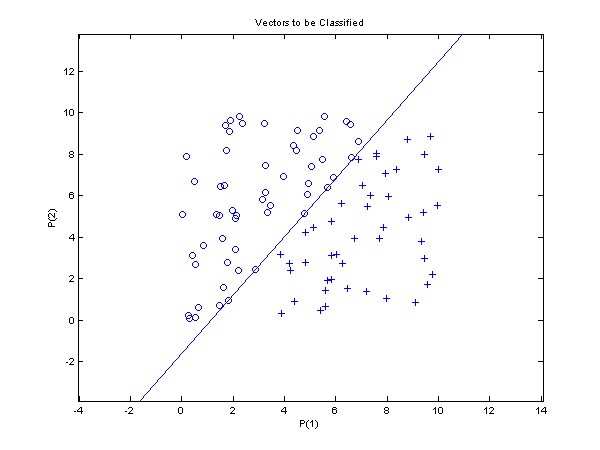
\includegraphics[scale=0.7]{figures/dane_a_data_learned.png}}
\caption{\label{fig:dane_a_data}Wykresy przedziału zestawu danych \texttt{dane\_a}}
\end{figure}

\begin{figure}[!h]
\centering
\subfigure[Wykres błędu (nie uczone)]{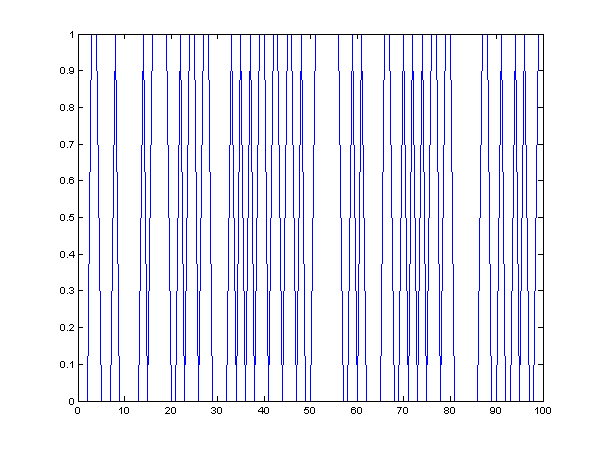
\includegraphics[scale=0.7]{figures/dane_1_error_unlearned.png}}
\subfigure[Wykres błędu (uczone)]{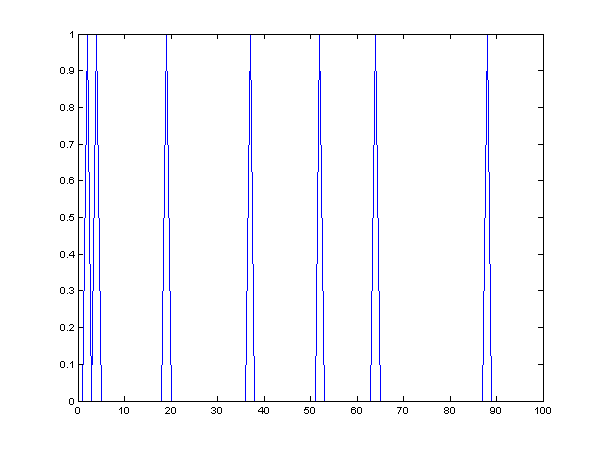
\includegraphics[scale=0.7]{figures/dane_1_error_learned.png}}
\caption{\label{fig:dane_1_error}Wykresy błędu zestawu danych \texttt{dane\_1}}
\end{figure}

\begin{figure}[!h]
\centering
\subfigure[Linia podziału (nie uczone)]{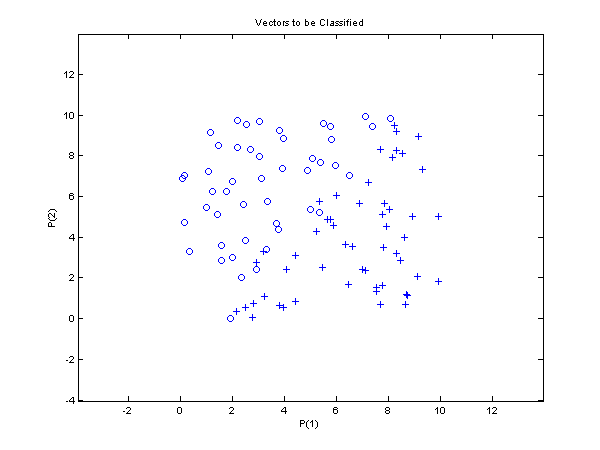
\includegraphics[scale=0.7]{figures/dane_1_data_unlearned.png}}
\subfigure[Linia podziału (uczone)]{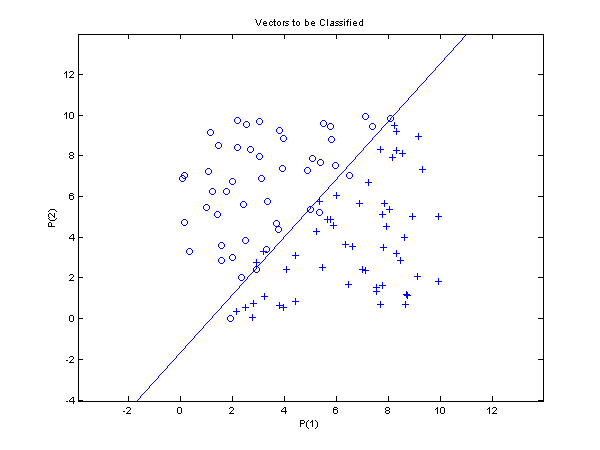
\includegraphics[scale=0.7]{figures/dane_1_data_learned.png}}
\caption{\label{fig:dane_1_data}Wykresy przedziału zestawu danych \texttt{dane\_1}}
\end{figure}

\begin{figure}[!h]
\centering
\subfigure[Wykres błędu (nie uczone)]{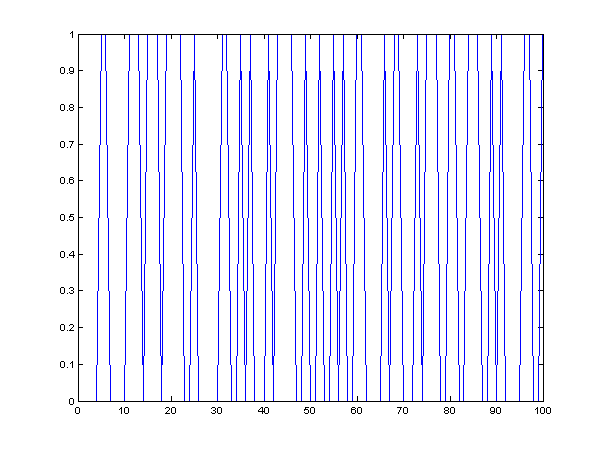
\includegraphics[scale=0.7]{figures/dane_2_error_unlearned.png}}
\subfigure[Wykres błędu (uczone)]{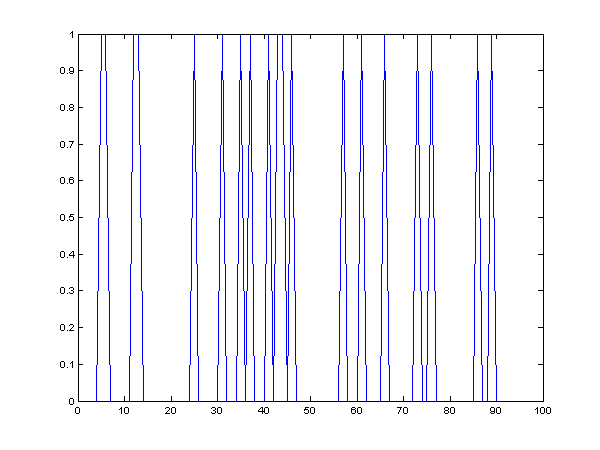
\includegraphics[scale=0.7]{figures/dane_2_error_learned.png}}
\caption{\label{fig:dane_2_error}Wykresy błędu zestawu danych \texttt{dane\_2}}
\end{figure}

\begin{figure}[!h]
\centering
\subfigure[Linia podziału (nie uczone)]{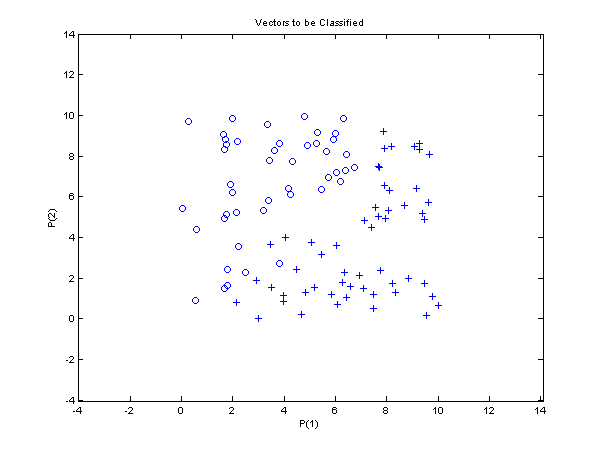
\includegraphics[scale=0.7]{figures/dane_2_data_unlearned.png}}
\subfigure[Linia podziału (uczone)]{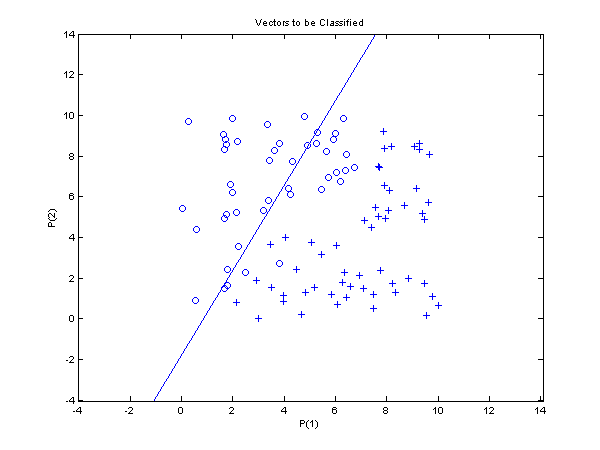
\includegraphics[scale=0.7]{figures/dane_2_data_learned.png}}
\caption{\label{fig:dane_2_data}Wykresy przedziału zestawu danych \texttt{dane\_2}}
\end{figure}

\begin{figure}[!h]
\centering
\subfigure[Wykres błędu (nie uczone)]{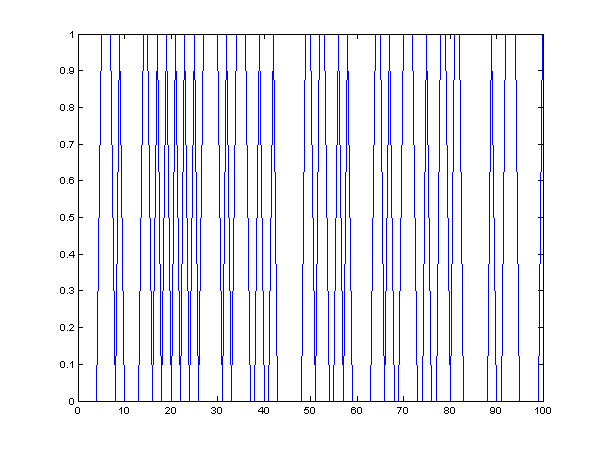
\includegraphics[scale=0.7]{figures/dane_3_error_unlearned.png}}
\subfigure[Wykres błędu (uczone)]{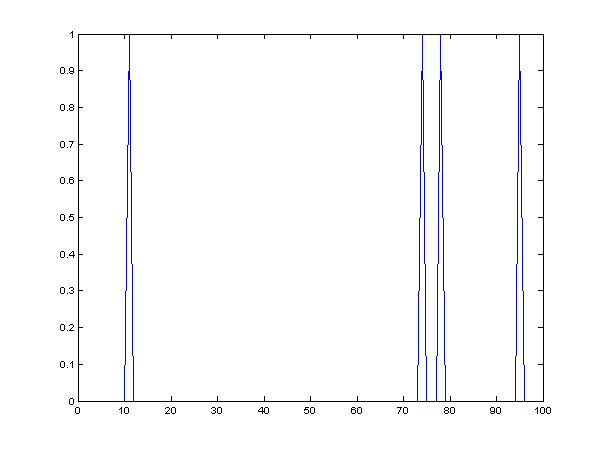
\includegraphics[scale=0.7]{figures/dane_3_error_learned.png}}
\caption{\label{fig:dane_3_error}Wykresy błędu zestawu danych \texttt{dane\_3}}
\end{figure}

\begin{figure}[!h]
\centering
\subfigure[Linia podziału (nie uczone)]{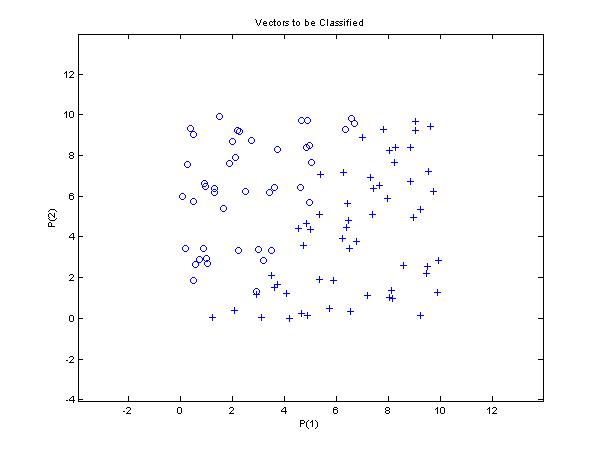
\includegraphics[scale=0.7]{figures/dane_3_data_unlearned.png}}
\subfigure[Linia podziału (uczone)]{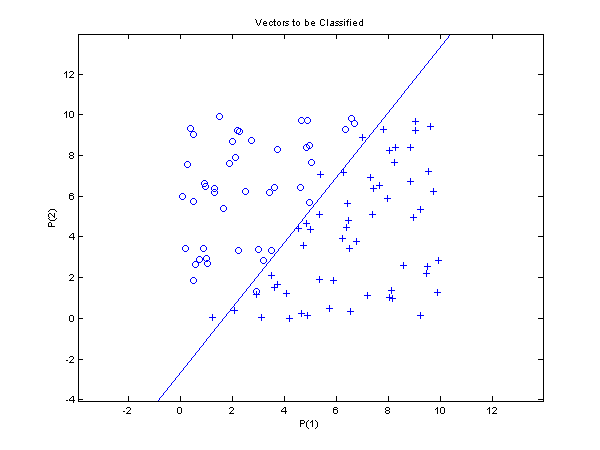
\includegraphics[scale=0.7]{figures/dane_3_data_learned.png}}
\caption{\label{fig:dane_3_data}Wykresy przedziału zestawu danych \texttt{dane\_3}}
\end{figure}

\begin{figure}[!h]
\centering
\subfigure[Wykres błędu (nie uczone)]{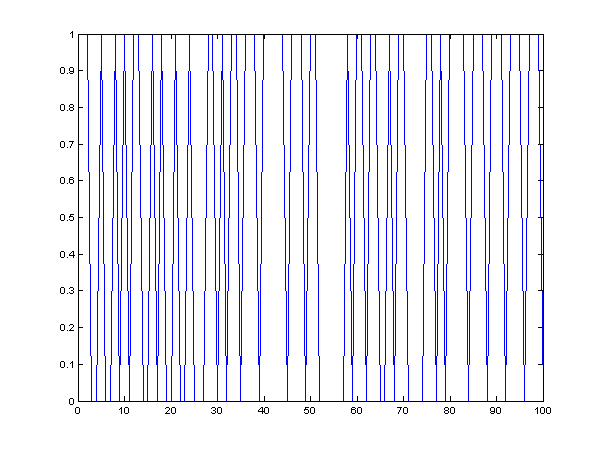
\includegraphics[scale=0.7]{figures/dane3d_a_error_unlearned.png}}
\subfigure[Wykres błędu (uczone)]{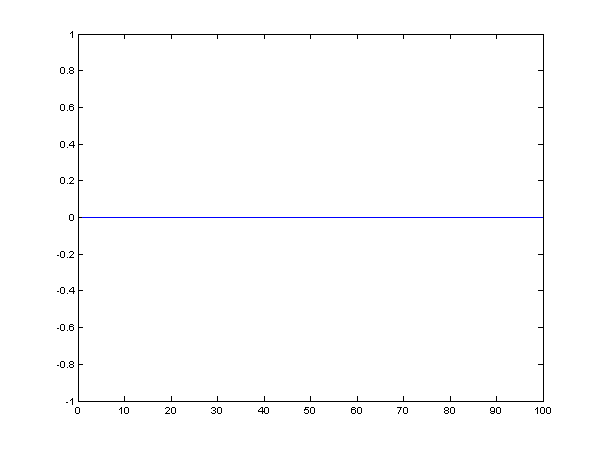
\includegraphics[scale=0.7]{figures/dane3d_a_error_learned.png}}
\caption{\label{fig:dane3d_a_error}Wykresy błędu zestawu danych \texttt{dane3d\_a}}
\end{figure}

\begin{figure}[!h]
\centering
\subfigure[Linia podziału (nie uczone)]{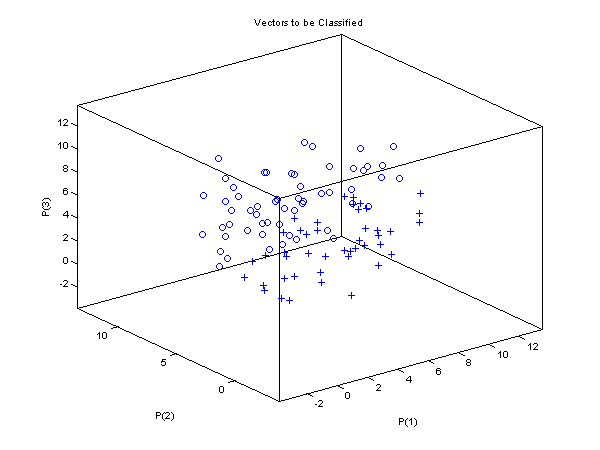
\includegraphics[scale=0.7]{figures/dane3d_a_data_unlearned.png}}
\subfigure[Linia podziału (uczone)]{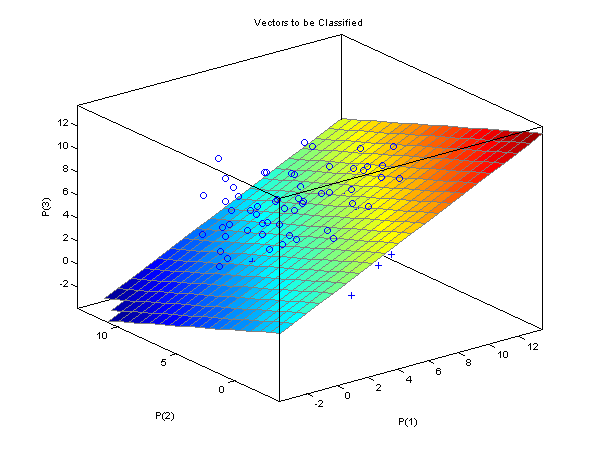
\includegraphics[scale=0.7]{figures/dane3d_a_data_learned.png}}
\caption{\label{fig:dane3d_a_data}Wykresy przedziału zestawu danych \texttt{dane3d\_a}}
\end{figure}

\begin{figure}[!h]
\centering
\subfigure[Wykres błędu (nie uczone)]{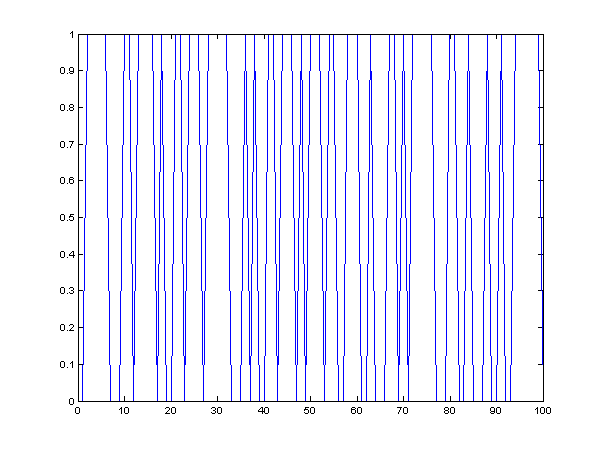
\includegraphics[scale=0.7]{figures/dane3d_1_error_unlearned.png}}
\subfigure[Wykres błędu (uczone)]{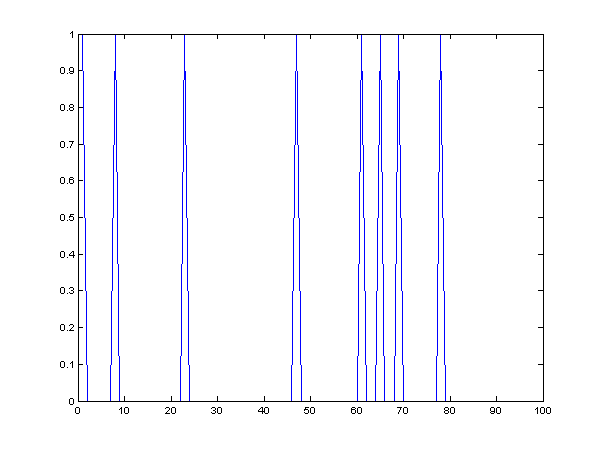
\includegraphics[scale=0.7]{figures/dane3d_1_error_learned.png}}
\caption{\label{fig:dane3d_1_error}Wykresy błędu zestawu danych \texttt{dane3d\_1}}
\end{figure}

\begin{figure}[!h]
\centering
\subfigure[Linia podziału (nie uczone)]{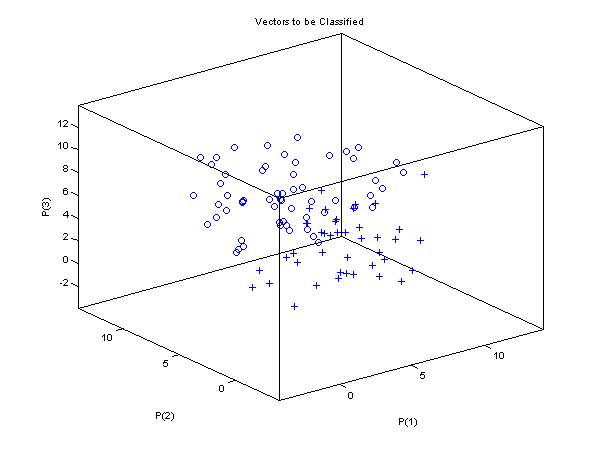
\includegraphics[scale=0.7]{figures/dane3d_1_data_unlearned.png}}
\subfigure[Linia podziału (uczone)]{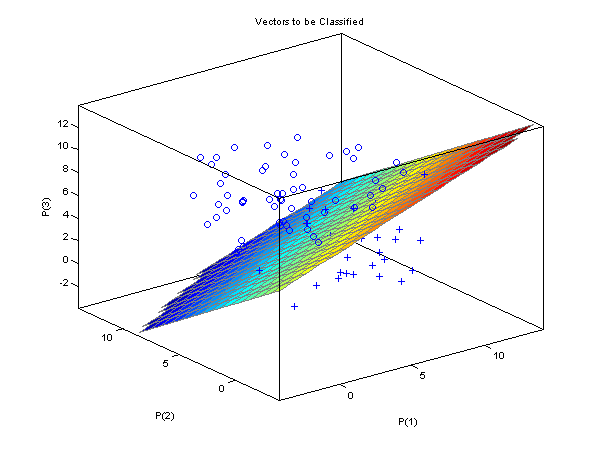
\includegraphics[scale=0.7]{figures/dane3d_1_data_learned.png}}
\caption{\label{fig:dane3d_1_data}Wykresy przedziału zestawu danych \texttt{dane3d\_1}}
\end{figure}

\begin{figure}[!h]
\centering
\subfigure[Wykres błędu (nie uczone)]{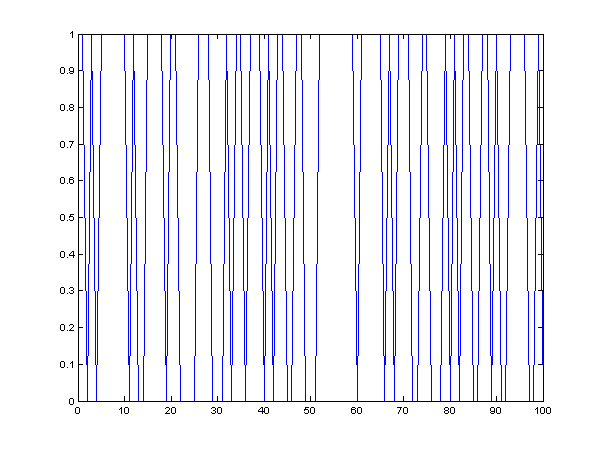
\includegraphics[scale=0.7]{figures/dane3d_2_error_unlearned.png}}
\subfigure[Wykres błędu (uczone)]{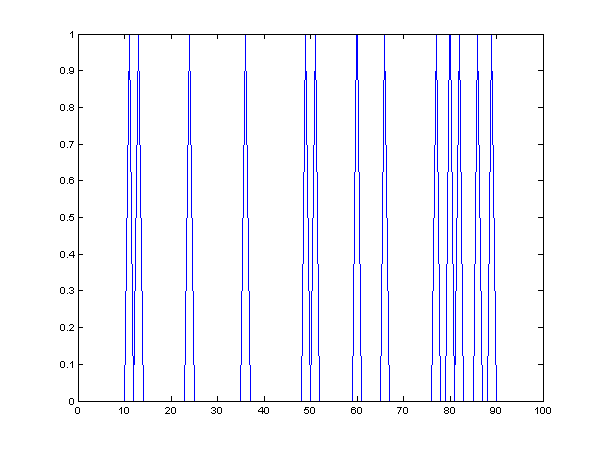
\includegraphics[scale=0.7]{figures/dane3d_2_error_learned.png}}
\caption{\label{fig:dane3d_2_error}Wykresy błędu zestawu danych \texttt{dane3d\_2}}
\end{figure}

\begin{figure}[!h]
\centering
\subfigure[Linia podziału (nie uczone)]{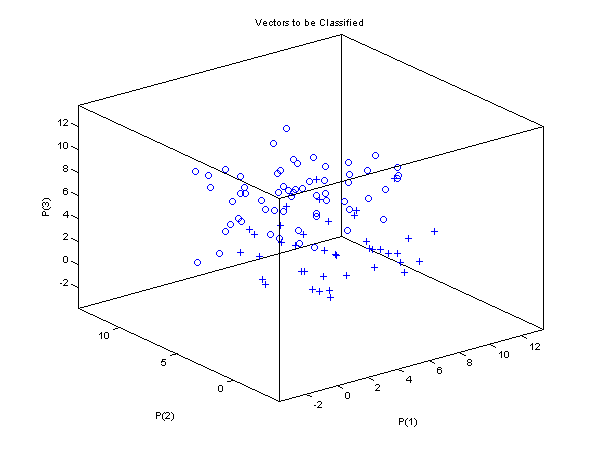
\includegraphics[scale=0.7]{figures/dane3d_2_data_unlearned.png}}
\subfigure[Linia podziału (uczone)]{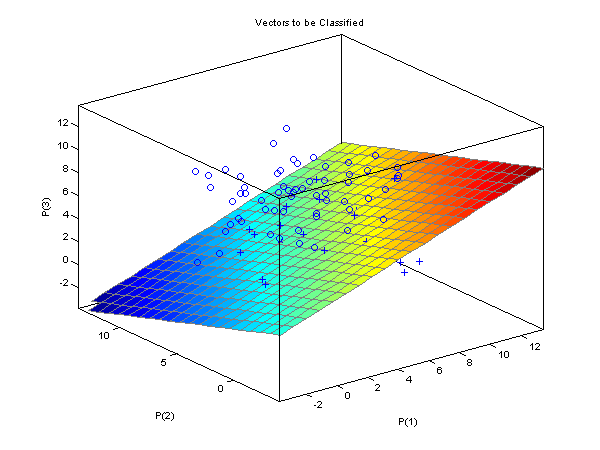
\includegraphics[scale=0.7]{figures/dane3d_2_data_learned.png}}
\caption{\label{fig:dane3d_2_data}Wykresy przedziału zestawu danych \texttt{dane3d\_2}}
\end{figure}

\begin{figure}[!h]
\centering
\subfigure[Wykres błędu (nie uczone)]{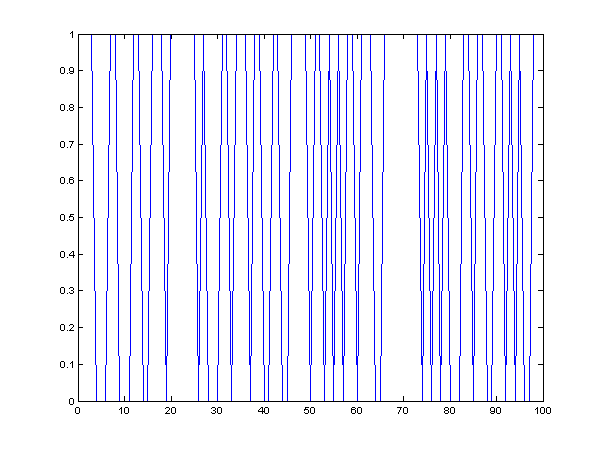
\includegraphics[scale=0.7]{figures/dane3d_3_error_unlearned.png}}
\subfigure[Wykres błędu (uczone)]{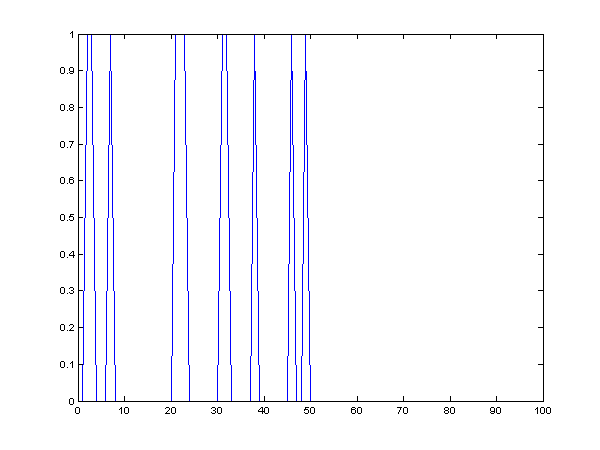
\includegraphics[scale=0.7]{figures/dane3d_3_error_learned.png}}
\caption{\label{fig:dane3d_3_error}Wykresy błędu zestawu danych \texttt{dane3d\_3}}
\end{figure}

\begin{figure}[!h]
\centering
\subfigure[Linia podziału (nie uczone)]{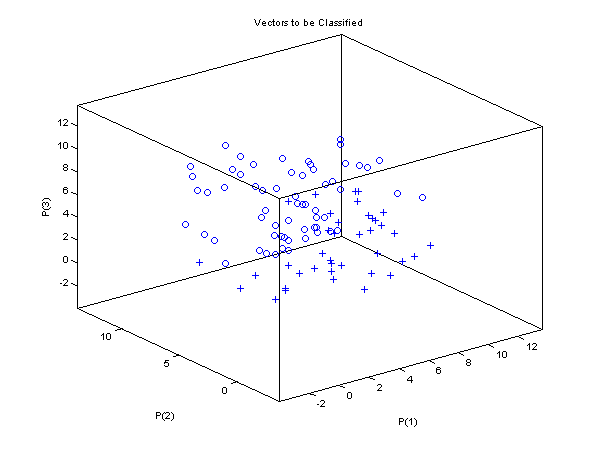
\includegraphics[scale=0.7]{figures/dane3d_3_data_unlearned.png}}
\subfigure[Linia podziału (uczone)]{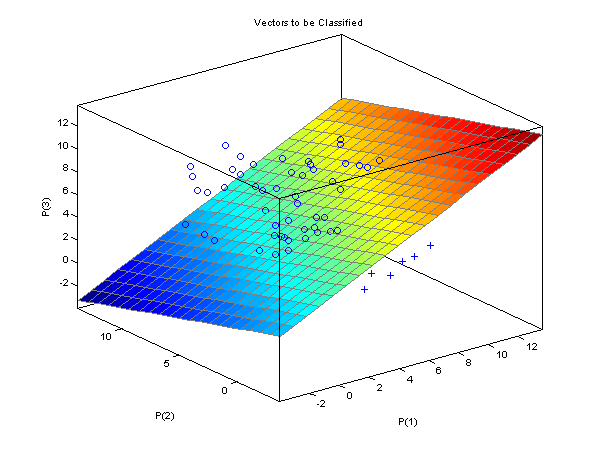
\includegraphics[scale=0.7]{figures/dane3d_3_data_learned.png}}
\caption{\label{fig:dane3d_3_data}Wykresy przedziału zestawu danych \texttt{dane3d\_3}}
\end{figure}

\clearpage
\begin{figure}[!h]
\centering
\subfigure[Wykres błędu (nie uczone)]{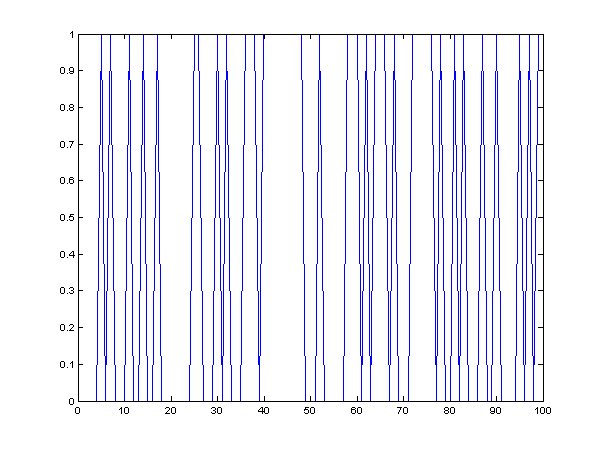
\includegraphics[scale=0.7]{figures/dane8d_a_error_unlearned.png}}
\subfigure[Wykres błędu (uczone)]{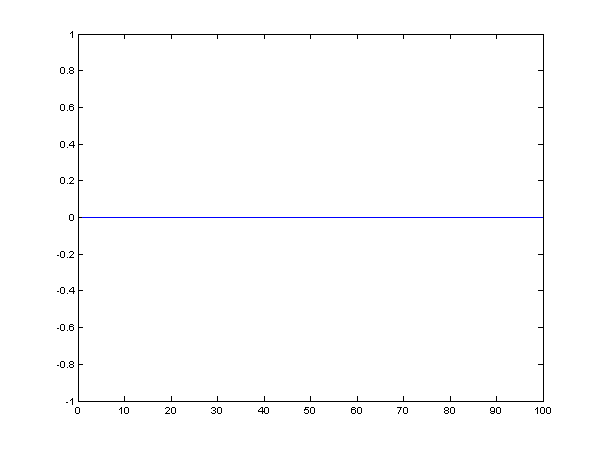
\includegraphics[scale=0.7]{figures/dane8d_a_error_learned.png}}
\caption{\label{fig:dane8d_a_error}Wykresy błędu zestawu danych \texttt{dane8d\_a}}
\end{figure}

\begin{figure}[!h]
\centering
\subfigure[Wykres błędu (nie uczone)]{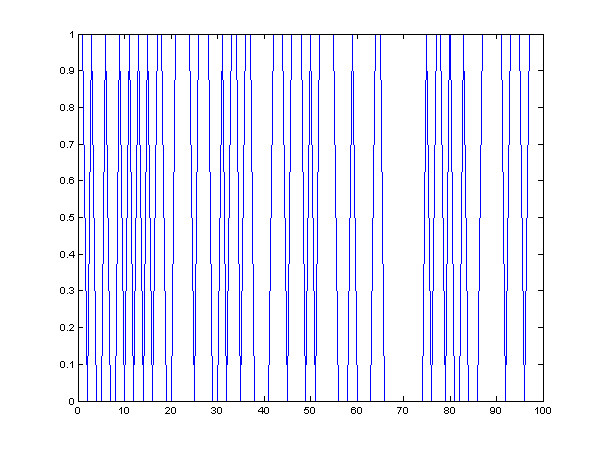
\includegraphics[scale=0.7]{figures/dane8d_2_error_unlearned.png}}
\subfigure[Wykres błędu (uczone)]{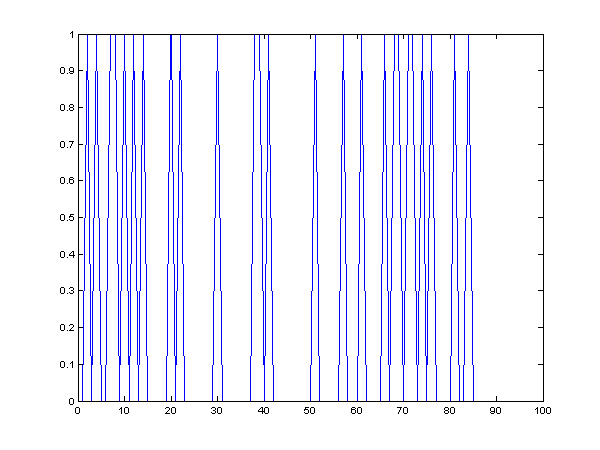
\includegraphics[scale=0.7]{figures/dane8d_2_error_learned.png}}
\caption{\label{fig:dane8d_2_error}Wykresy błędu zestawu danych \texttt{dane8d\_2}}
\end{figure}

\begin{figure}[!h]
\centering
\subfigure[Wykres błędu (nie uczone)]{\includegraphics[scale=0.7]{figures/dane8d_3_error_unlearned.png}}
\subfigure[Wykres błędu (uczone)]{\includegraphics[scale=0.7]{figures/dane8d_3_error_learned.png}}
\caption{\label{fig:dane8d_3_error}Wykresy błędu zestawu danych \texttt{dane8d\_3}}
\end{figure}

\begin{figure}[!h]
\centering
\subfigure[Wykres błędu (nie uczone)]{\includegraphics[scale=0.7]{figures/dane8d_1_error_unlearned.png}}
\subfigure[Wykres błędu (uczone)]{\includegraphics[scale=0.7]{figures/dane8d_1_error_learned.png}}
\caption{\label{fig:dane8d_1_error}Wykresy błędu zestawu danych \texttt{dane8d\_1}}
\end{figure}

\clearpage
\section{Opracowanie własnej uczącą neuron z wykorzystaniem reguły delta}
\subsection{Opis funkcji \texttt{delta}}
Zrealizowany algorytm opiera się na neuronie według wzoru \ref{eq:1} i jest widoczny w listingu \ref{lst:delta.m}. Dane wejściowe $x_0, x_1, \cdots, x_n$ są wczytane zmienną \texttt{in}.

Neuron posiada na wyjściu wartość $y=1$ albo $y=0$ kiedy funkcja aktywacyjna $\varphi$ jest większa lub równa albo mniejsza od wartości $\theta$. Oczekiwane wartości wyjściowe są wczytane zmienną \texttt{out}. Uczone wartości wyjściowe są oddane zmienną \texttt{learned}.

\begin{equation}
\label{eq:1}
\begin{array}{rcll}
y & = & \left\{
    \begin{array}{lc}
        1 & \varphi \ge \theta \\
        0 & \varphi < \theta \\
    \end{array}
\right. & \textrm{gdzie} \\
\\
\theta & = & 0 \\
\varphi & = & w_0 x_0 + w_1 x_1 + \cdots + w_n x_n + w_{n+1} b \\
b & = & 1 \\
\end{array}
\end{equation}

Wartości początkowe wag $W_0 = (w_0, w_1, \cdots , w_n)$ są wybrane przypadkowo i leżą między $[0,1]$ (linia 20 listingu \ref{lst:delta.m}). W każdej iteracji epoki uczenia są korygowane wartości wag według wzoru \ref{eq:2} (linia 55 listingu \ref{lst:delta.m}). Zmienna $0 > \eta \ge 1$ stanowi parametr uczący i jego wartość została w tym przypadku wybrana jako $\eta = 0.2$.

$\delta$ jest różnicą między uczonymi wartościami $t$ danej epoki i wartościami wejściowymi $y$ (linia 49 listingu \ref{lst:delta.m}). Uczone dane $t$ w bierzącej epoce są wyliczane za pomocą aktualnej sumy wag i zastosowania wzoru \ref{eq:1} (linie 36-46 listingu \ref{lst:delta.m}).

\begin{equation}
\label{eq:2}
\begin{array}{rcll}
W_{i} & = & W_{i-1} + \Delta W & \textrm{gdzie} \\
\\
\Delta W & = & \eta \ \delta \ x \\
\\
\eta & = & 0.2 \\
\delta & = & t-y \\
x & = & (x_0, x_1, \cdots, x_n, b)
\end{array}
\end{equation}

Iteracyjnie wagi $W$ w każdej epoce są korygowane aż do momentu kiedy $t = y$ lub kiedy aktualna epoka jest równa maksymalnej epoce danej jako parametr \texttt{epochs} (linia 26/59 listingu \ref{lst:delta.m}).

Następnie pomocnicza funkcja została zaimplementowana aby ułatwić współprace z plikami. Kod jest widoczny w listingu \ref{lst:load_delta.m}.

Kod został napisany w środowisku Octave 3.0.5 pod Linux ze względu na fakt że to jest środowisko Open Source i za tym o wiele łatwej dostępne od pakietu Matlab.

\begin{center}
\lstset{captionpos=b,caption={\texttt{load\_delta.m}: Funkcja pomocnicza dla reguły delta},label=lst:load_delta.m}
\lstinputlisting{src/load_delta.m}
\end{center}

\begin{table}[h!]
\centering
\begin{tabular}[t]{l|p{0.5\textwidth}|c|c}
Dane (prefiks) & Wagi & Epoki & Udane uczenie \\
\hline
\texttt{percep} & 0.15562   0.95492  -3.27467 & 15 & Tak \\
\texttt{dane\_a} & 11.6389   -8.2880  -13.2825 & 48 & Tak \\
\texttt{dane\_1} & 10.2720   -8.7994  -15.0422 & N/A & Nie \\
\texttt{dane\_2} & 10.9469   -5.8266  -13.2175 & N/A & Nie \\
\texttt{dane\_3} & 10.4504   -5.2809  -17.7526 & N/A & Nie  \\
\texttt{dane3d\_a} & 7.2781   -4.3285  -11.2311   32.8859 & 122 & Tak \\
\texttt{dane3d\_1} & 6.4942   -6.7073  -10.0775   45.8484 & N/A & Nie \\
\texttt{dane3d\_2} & 6.9544   -4.0883  -11.7865   27.7291 & N/A & Nie \\
\texttt{dane3d\_3} & 8.3543   -3.3688  -12.0120   38.4670 & N/A & Nie  \\
\texttt{dane8d\_a} & 10.4484    12.2477    11.1905    12.3418    11.5381    13.3448    10.0944     9.6301  -448.6094 & 3995 & Tak  \\
\texttt{dane8d\_1} & 9.7304     5.4700     7.8741    10.3601     7.2305     7.1548     9.8148    4.8561  -342.2336 & N/A & Nie \\
\texttt{dane8d\_2} & 5.7690     6.5841     9.0588    13.3850     6.2696     9.8061     3.6560    11.1488  -361.6779 & N/A & Nie \\
\texttt{dane8d\_3} & 6.9226     7.9210     4.8611     8.3132     9.8582     4.9881    11.4248    11.2508  -333.1923 & N/A & Nie \\
\end{tabular}
\caption{\label{tab:wyniki_bada}Wyniki badan własną implementacją reguły delta}
\end{table}

Można zauważyć w badaniach własną funkcją delta że ilość epok (iteracji algorytmu) zwiększa się z większą ilością parametrów.

\clearpage
\subsection{Kod funkcji \texttt{delta}}

\begin{center}
\lstset{numbers=left,captionpos=b,caption=\texttt{delta.m}: Funkcja ucząca neuron regułą delta,label=lst:delta.m}
\lstinputlisting{src/delta.m}
\end{center}

\end{document}

